\documentclass[11pt,a4paper]{article}
\usepackage{amsmath, tabularx, geometry, graphicx, xcolor, multirow}

\usepackage{tikz, listings}
\usepackage{xcolor}

\usetikzlibrary{positioning}
\newdimen\nodeDist
\nodeDist=35mm

\geometry{a4paper, left=20mm, top=20mm}
\graphicspath{{./imgs/}}
\renewcommand\tabularxcolumn[1]{m{#1}}

\title{Aprendizagem 2021/22 Homework I - Group 66}
\author{João Cardoso, 99251. José João Ferreira, 99259}

\begin{document}

\color{darkgray}
\hspace{-8.25mm}
\begin{tabularx}{1.09\textwidth} {>{\raggedright\arraybackslash}X >{\centering\arraybackslash}X >{\raggedleft\arraybackslash}X}
  
\includegraphics[scale=0.2]{tecnico.pdf} &
  \textbf{Aprendizagem 2022/23} \par \textbf{Homework I - Group 66} &
  João Cardoso, 99251 \par José João Ferreira, 99259
\end{tabularx}
\color{black}

\begin{center}
\textbf{I. Pen-and-paper}
\end{center}

% PROBLEM 1
\begin{flushleft}
\textbf{1)}
\small
\begin{tabular}{llcc}
                                                  &                        & \multicolumn{2}{c}{Real}                        \\ \cline{3-4} 
                                                  & \multicolumn{1}{l|}{}  & \multicolumn{1}{c|}{P} & \multicolumn{1}{c|}{N} \\ \cline{2-4} 
  \multicolumn{1}{c|}{\multirow{2}{*}{Predicted}} & \multicolumn{1}{c|}{P} & \multicolumn{1}{c|}{8} & \multicolumn{1}{c|}{4} \\ \cline{2-4} 
  \multicolumn{1}{c|}{}                           & \multicolumn{1}{c|}{N} & \multicolumn{1}{c|}{3} & \multicolumn{1}{c|}{5} \\ \cline{2-4} 
\end{tabular}

\normalsize
\end{flushleft}

% PROBLEM 2
\begin{flushleft}
\textbf{2)}
\small
\hspace{-8.25mm}
\vspace{4mm}
\begin{tabularx}{1.09\textwidth}{XXX}
  
  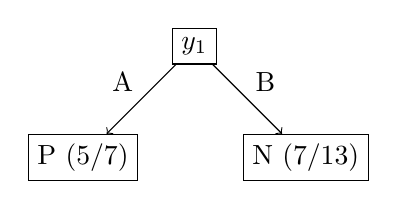
\begin{tikzpicture}[node/.style={draw,rectangle}, ->]
    \node [node] (node_1) {$y_1$};
    \path (node_1) ++ (-135:2) node [node] (node_2) {P (5/7)};
    \path (node_1) ++ (-45:2) node [node] (node_3) {N (7/13)};
    \draw (node_1) -- (node_2) node [left,pos=0.25] {A\hspace{2mm} }(node_1);
    \draw (node_1) -- (node_3) node [right,pos=0.25] {\hspace{2mm}B}(node_1);
  \end{tikzpicture} &

  \begin{tabular}{llcc}
    &                        & \multicolumn{2}{c}{Real}                        \\ \cline{3-4} 
    & \multicolumn{1}{l|}{}  & \multicolumn{1}{c|}{P} & \multicolumn{1}{c|}{N} \\ \cline{2-4} 
  \multicolumn{1}{c|}{\multirow{2}{*}{Predicted}} & \multicolumn{1}{c|}{P} & \multicolumn{1}{c|}{5} & \multicolumn{1}{c|}{2} \\ \cline{2-4} 
  \multicolumn{1}{c|}{}                           & \multicolumn{1}{c|}{N} & \multicolumn{1}{c|}{5} & \multicolumn{1}{c|}{7} \\ \cline{2-4} 
  \end{tabular} &
  \normalsize
  $ Precision = \frac{TP}{TP + FP} = \frac{5}{5 + 2} = \frac{5}{7} $ \par
  $ Recall = \frac{TP}{TP + FN} = \frac{5}{5 + 5} = \frac{1}{2} $
\end{tabularx}
\vspace{0mm}
\normalsize
$ F_{\beta = 1} = \frac{1}{\frac{1}{2Precision} + \frac{1}{2Recall}} = \frac{1}{\frac{7}{10} + \frac{2}{2}} = \frac{1}{\frac{17}{10}} = \frac{10}{17} \approx 0.588235 $ \par
\end{flushleft}
\vspace*{2mm}

% PROBLEM 3
\begin{flushleft}
\textbf{3)}
Some values of $y_2$, given $y_1 = A$, might be missing or corrupted and it could be risky to train the system with corrupt or incomplete data. Another reason could be a very low information gain about $y_{out}$ of the variable $y_2$, given $y_1 = A$, and therefore it would be a waste of time to train the system with this variable. \par
\end{flushleft}
\vspace*{2mm}

% PROBLEM 4
\begin{flushleft}
\textbf{4)}
\small
\hspace{-8.25mm}
\begin{tabularx}{1.09\textwidth}{>{\hsize=.25\hsize}X X}
  \vspace{-17.5mm}
  \begin{tabular}{ccc}
  $y_1$ & $y_2$                 & $y_{out}$ \\ \hline
  A     &                       & P         \\ \hline
  A     &                       & P         \\ \hline
  A     &                       & P         \\ \hline
  A     &                       & P         \\ \hline
  A     &                       & P         \\ \hline
  A     &                       & N         \\ \hline
  A     &                       & N         \\ \hline
  B     & \textgreater 2        & P         \\ \hline
  B     & \textgreater 2        & P         \\ \hline
  B     & \textgreater 2        & P         \\ \hline
  B     & \textgreater 2        & N         \\ \hline
  B     & \textgreater 2        & N         \\ \hline
  B     & \textgreater 2        & N         \\ \hline
  B     & \textgreater 2        & N         \\ \hline
  B     & \textgreater 2        & N         \\ \hline
  B     & $\leq$2               & P         \\ \hline
  B     & $\leq$2               & P         \\ \hline
  B     & $\leq$2               & P         \\ \hline
  B     & $\leq$2               & N         \\ \hline
  B     & $\leq$2               & N         \\
  \end{tabular} &
  
  \normalsize\vspace{5mm}
  $ E(y) = -\sum_{v \in y} P(v)\log_2(P(v)) $
  \newline\newline
  $ E(y_{out}) = -\frac{11}{20}\log_2(\frac{11}{20}) -\frac{9}{20}\log_2(\frac{9}{20}) $ \par\vspace{1mm}
  \hspace{12.25mm} $ \approx 0.992774 $
  \newline\newline
  $ E(y_{out}|y_1) = \frac{7}{20}[-\frac{5}{7}\log_2(\frac{5}{7}) -\frac{2}{7}\log_2(\frac{2}{7})] + \frac{13}{20}[-\frac{7}{13}\log_2(\frac{7}{13}) -\frac{6}{13}\log_2(\frac{6}{13})] $ \par\vspace{1mm}
  \hspace{16.75mm} $ \approx 0.949315 $ 
  \newline\newline
  $ IG(y_{out}|y_1) = E(y_{out}) - E(y_{out}|y_1) $ \par\vspace{1mm}
  \hspace{18.75mm} $ = 0.992774 - 0.949315 $ \par\vspace{1mm}
  \hspace{18.75mm} $ = 0.043459 $
  
\end{tabularx}
\end{flushleft}

\pagebreak

\color{darkgray}
\hspace{-8.25mm}
\begin{tabularx}{1.09\textwidth} {>{\raggedright\arraybackslash}X >{\centering\arraybackslash}X >{\raggedleft\arraybackslash}X}
  
\includegraphics[scale=0.2]{tecnico.pdf} &
  \textbf{Aprendizagem 2022/23} \par \textbf{Homework I - Group 66} &
  João Cardoso, 99251 \par José João Ferreira, 99259
\end{tabularx}
\color{black}

\begin{center}
\textbf{II. Programming}
\end{center}

% PROBLEM 1
\begin{flushleft}
\textbf{1)} \par
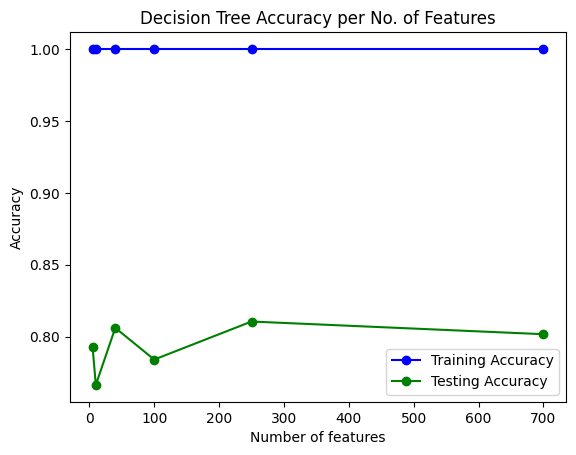
\includegraphics[scale=0.75]{plot.png}
\end{flushleft}
\vspace*{2mm}

% PROBLEM 2
\begin{flushleft}
\textbf{2)}
From the plot above, we can see that the decision tree is overfitting the training data as the training accuracy is always 1.

Overfitting is the phenomenon in which the learning system tightly fits the given training data so much that it would be 100\% accurate in predicting the outcomes of the trained data, if run through the system again.

This has happened because the generated decision tree has no depth limit and, as such, perfectly fits all samples in the training data set. Because it covers all cases down to the most singular one, the training accuracy is 1.

The results show that the mean of testing accuracy values is approximately 0.794, which is considerably less than 1. This is legitimate, given that the tree has been trained with the training data in such detail that it cannot accurately predict the outcomes of the untrained data. This is one of the biggest problems of Overfitting.
\end{flushleft}

\pagebreak

\color{darkgray}
\hspace{-8.25mm}
\begin{tabularx}{1.09\textwidth} {>{\raggedright\arraybackslash}X >{\centering\arraybackslash}X >{\raggedleft\arraybackslash}X}
  
\includegraphics[scale=0.2]{tecnico.pdf} &
  \textbf{Aprendizagem 2022/23} \par \textbf{Homework I - Group 66} &
  João Cardoso, 99251 \par José João Ferreira, 99259
\end{tabularx}
\color{black}

\begin{center}
\textbf{III. Appendix}
\end{center}

\definecolor{codegreen}{rgb}{0,0.6,0}
\definecolor{codegray}{rgb}{0.5,0.5,0.5}
\definecolor{codepurple}{rgb}{0.58,0,0.82}
\definecolor{backcolour}{rgb}{0.95,0.95,0.92}
\lstdefinestyle{mystyle}{
    backgroundcolor=\color{backcolour},   
    commentstyle=\color{codegreen},
    keywordstyle=\color{magenta},
    numberstyle=\tiny\color{codegray},
    stringstyle=\color{codepurple},
    basicstyle=\ttfamily\footnotesize,
    breakatwhitespace=false,         
    breaklines=true,                 
    captionpos=b,                    
    keepspaces=true,                 
    numbers=left,                    
    numbersep=5pt,                  
    showspaces=false,                
    showstringspaces=false,
    showtabs=false,                  
    tabsize=2}
\lstset{style=mystyle}

\lstinputlisting[language=Python]{pd_speech.py}

\end{document}